% Adding a coloured vertical edge to the pages in the chapter
\ClearShipoutPicture
\AddToShipoutPicture{%
  \AtPageLowerLeft{%
    \checkoddpage
    \ifoddpage
      \begin{tikzpicture}[remember picture,overlay] % Odd page → right edge
        \draw[line width=80pt, colour_chapter7] 
             (\paperwidth,0) -- (\paperwidth,\paperheight);
      \end{tikzpicture}%
    \else
      \begin{tikzpicture}[remember picture,overlay] % Even page → left edge
        \draw[line width=80pt, colour_chapter7] 
             (0,0) -- (0,\paperheight);
      \end{tikzpicture}%
    \fi
  }%
}

%%%%%%%%%%%%%%%%%%%%%%%%%%%%%%%%%%%%%%%%%%%%%%%%%%%%%%%%%%%%%
\chapter{Towards predictions over a continuous global domain: 
global implementation of the regionally-trained models}
\label{regional_to_global_training}
\graphicspath{{chapter_07/figures}{chapter_07/tables}}
%%%%%%%%%%%%%%%%%%%%%%%%%%%%%%%%%%%%%%%%%%%%%%%%%%%%%%%%%%%%%

\underline{\textbf{Authors' contribution for this chapter:}} Fatima M. Pillosu designed the study, with advice from Hannah Cloke and Christel Prudhomme, obtained the datasets, carried out the analysis, and led the writing of the manuscript. All authors assisted with writing the manuscript. Overall, 90\% of the writing was undertaken by Fatima M. Pillosu.

\vspace{\baselineskip}

\section*{PREFACE}
\addcontentsline{toc}{section}{PREFACE}

The first main analysis chapter (Chapter \ref{flash_flood_focused_verification_rainfall_based_ff}) undertakes the flash-flood-focused evaluation of short- and medium-range post-processed probabilistic point-scale rainfall forecasts. Such forecasts have been shown to predict better than the raw ERA5 flash-flood-triggering localised extreme rainfall events \citep{Pillosu_2025a}. While such an improvement in the prediction of localised extreme rainfall should enable the improved detection of areas at risk of flash floods, a flash-flood-focused assessment is fundamental to determining the extent to which enhanced rainfall prediction accuracy translates into meaningful improvements in flash flood hazard identification. In this chapter, \textcolor{colour_chapter7}{research question 1 (RQ1) "Can post-processed global NWP rainfall forecasts successfully identify areas at risk of flash floods up to medium-range lead times?"} is answered. Moreover, the first research component of this thesis is addressed, i.e. \textcolor{colour_chapter5}{developing a flash-flood-focused verification framework for predictions of areas at risk of flash floods, designed to benchmark the capability of different predictive systems}. Hence, this evaluation establishes a performance benchmark against which more sophisticated modelling approaches - incorporating additional hydrological and topographical parameters - can be measured. Such comparative analysis is essential for determining whether the increased computational demands and data requirements of complex systems yield commensurate improvements in flash flood prediction accuracy, or whether simpler precipitation-based approaches provide sufficient utility for early warning applications.

\clearpage

\section*{ABSTRACT}
\addcontentsline{toc}{section}{ABSTRACT}

\clearpage



%%%%%%%%%%%%%%%%%%%%%%
\section{Introduction}


%%%%%%%%%%%%%%
\section{Data}


%%%%%%%%%%%%%%%%%
\section{Methods}


%%%%%%%%%%%%%%%%%
\section{Results}

\subsection{Extension of regional training to global application}

\begin{figure}[htbp]
\centering
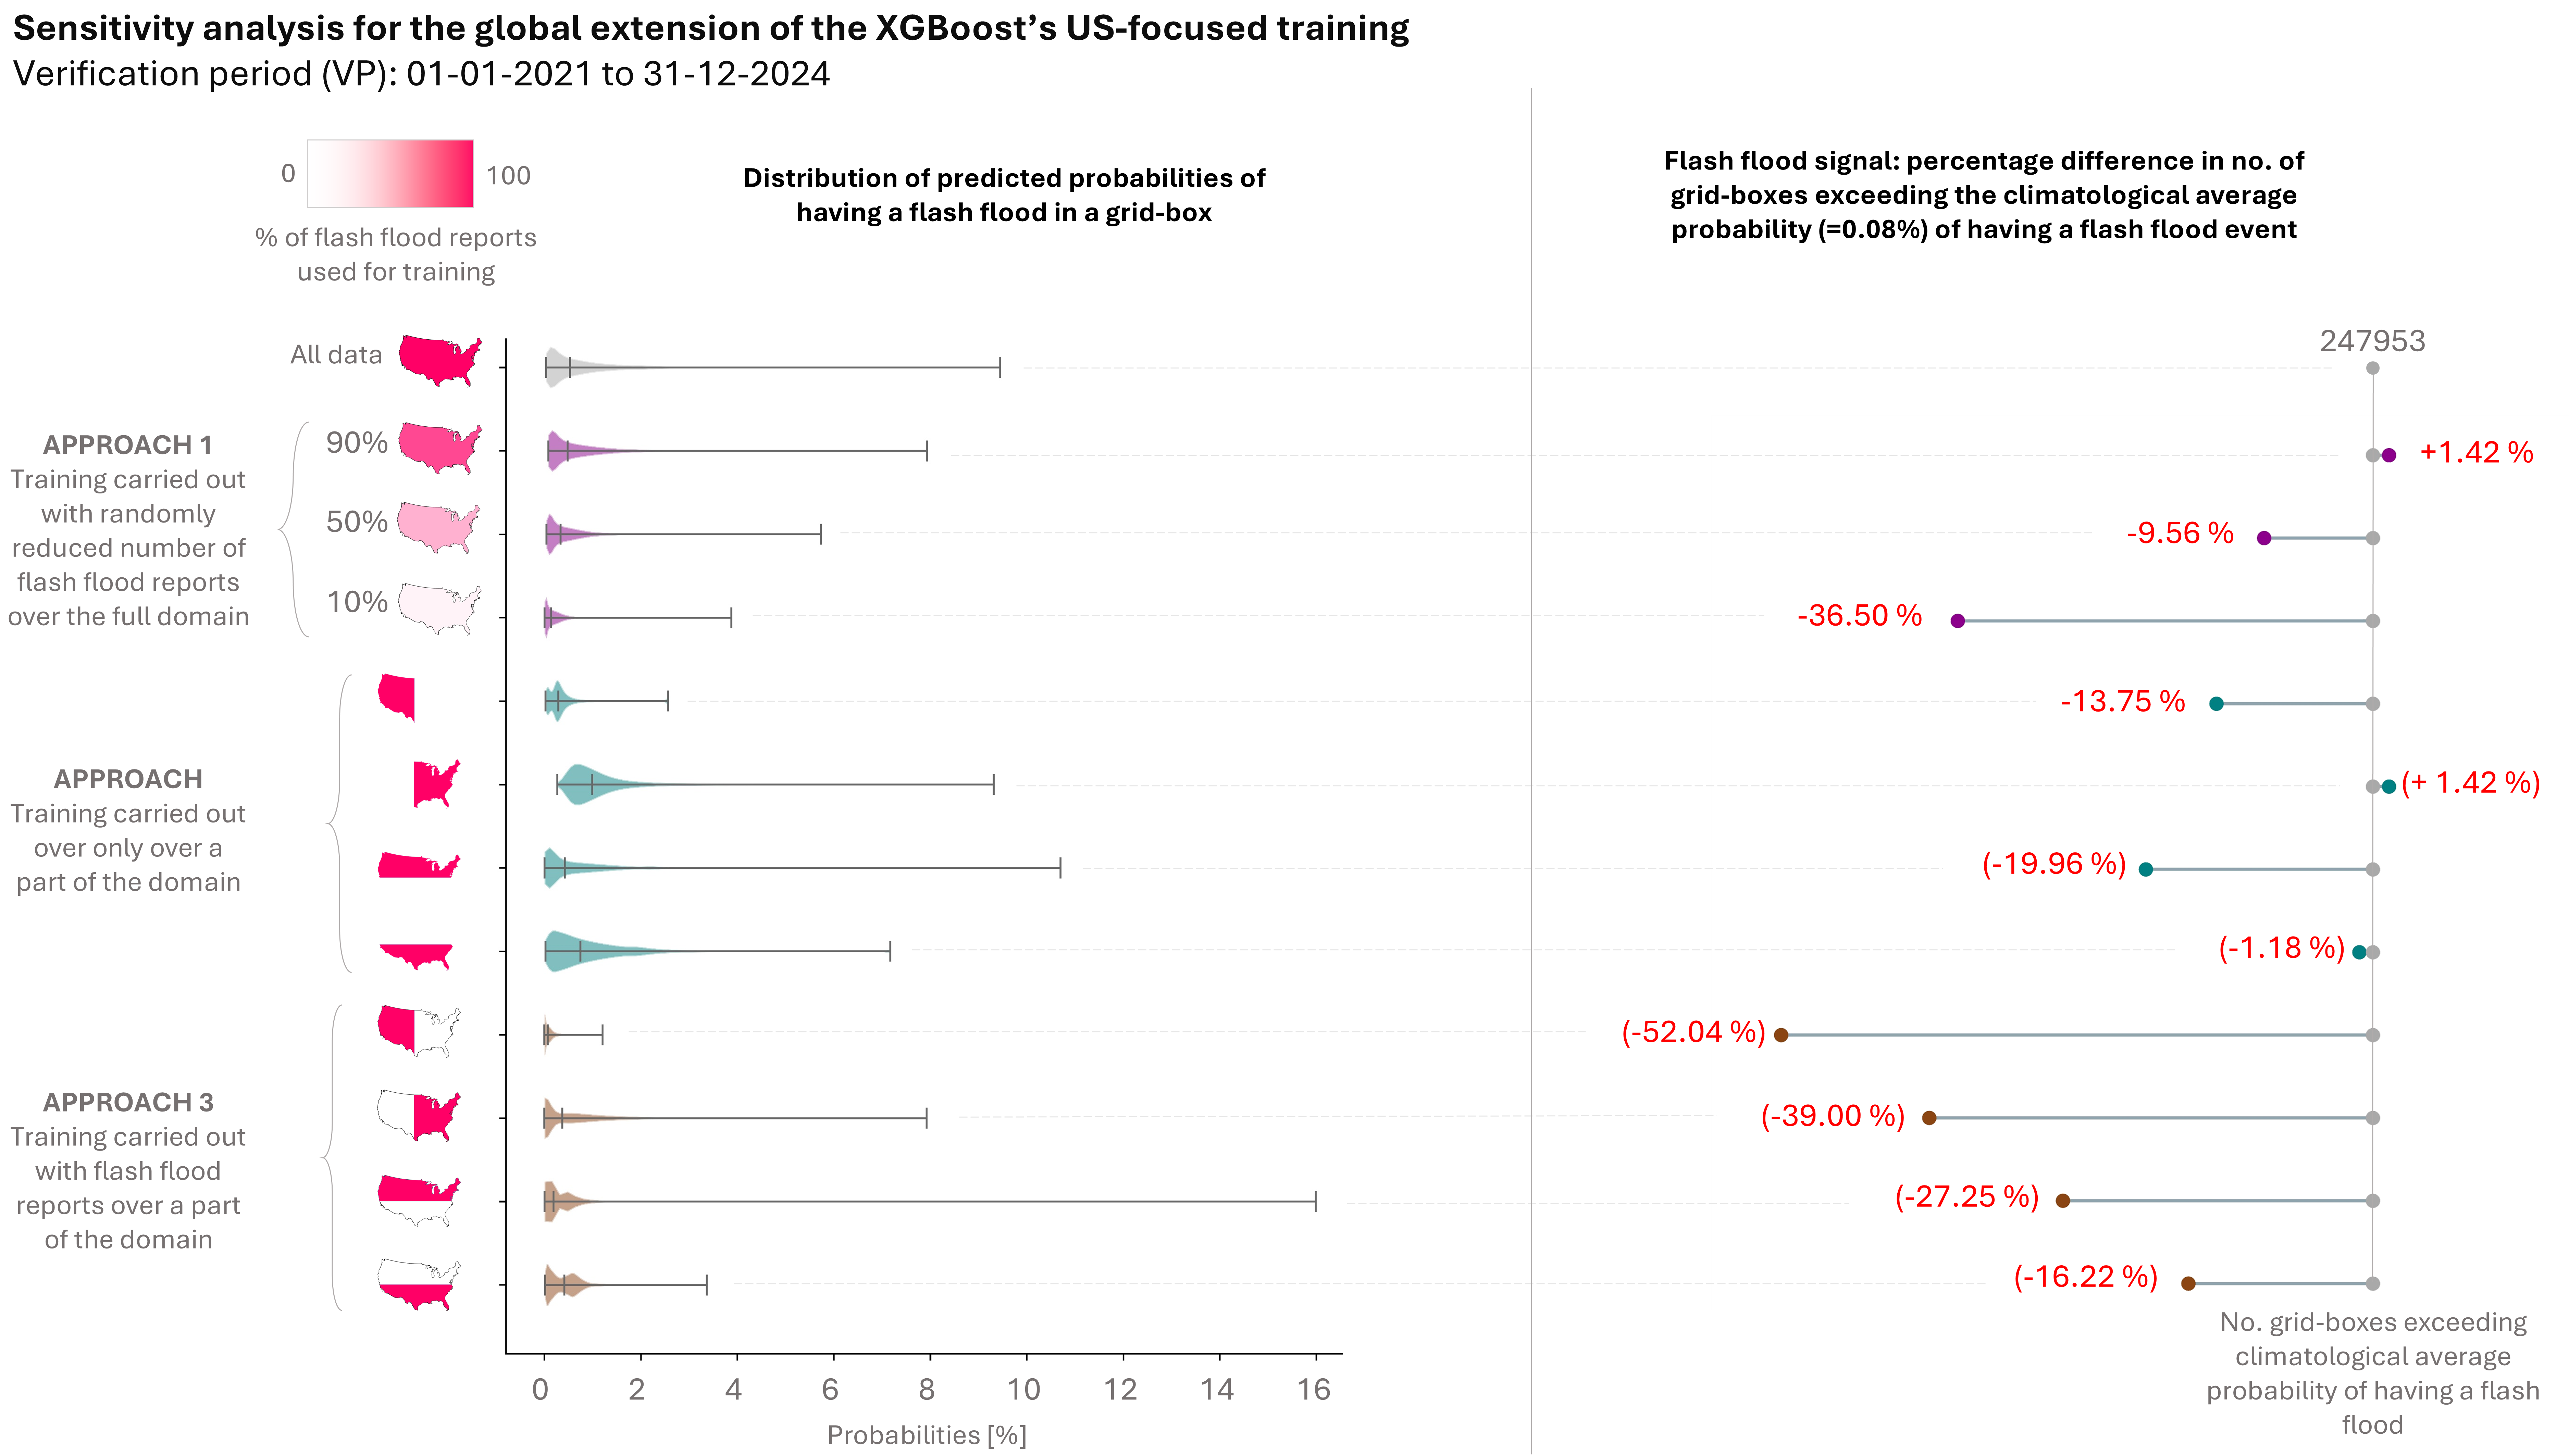
\includegraphics[width=\textwidth]{sensitivity_analysis_global_extension.png}
\caption{\textbf{Global extension performance of regionally-trained XGBoost under different U.S. training data sampling strategies.} Violin plots show predicted probability distributions, whilst dots indicate percentage change in flash flood detection capability relative to climatological baseline. Three approaches tested: random sampling (Approach 1), domain-restricted training (Approach 2), and sub-regional training (Approach 3).}
\label{fig:sensitivity_analysis_global_extension}
\end{figure}

The global application of the regionally-trained XGBoost was evaluated through three distinct approaches, each employing different spatial sampling strategies for training data inclusion (Figure \ref{fig:sensitivity_analysis_global_extension}). The baseline configuration utilising all available flash flood reports in the Storm Event Database, within the verification period, produced a conservative probability distribution, with most predictions remaining below 10\% and 247,953 grid boxes exceeding the climatological average flash flood probability (0.08\%).

Approach 1, which implemented a random reduction of the flash flood reports to predetermined percentages (90\%, 50\%, and 10\%) uniformly, across the entire U.S. domain, demonstrated variable performance. The 90\% sampling configuration merginally increased the detection capability (i.e. number of flash flood reports exceeding the climatological average of flash flood events) by 1.42\%, while the 50\% and the 90\% reductions showed, respectively, a degradation of 9.56\% and 36.50\%, suggesting non-linear relationships between training data volumes and model performance.

Approach 2 explored a spatially-constrained training strategy where the model was trained only over a certain part of the domain where observations are available. The model did not see at all the other part of the domain, and it was applied to create predictions over the whole CONUS domain. This approach simulates a global training that considers only those areas of the world with good observations during training, but uses the model globally to create predictions over the continuous global domain. The reduction in the predicted probabilities was the smallest over the three approaches, with the biggest  reductions of -13.75\% and -19.96\% when the model was trained using the parts of the domain with the smallest number of flash flood reports i.e., the east and the north, respectively. When using the parts of the domain with the biggest number of reports, i.e., the west and the south, there was an increase of +1.42\% and a minimal reduction of -1.18\% of grid-boxes with a flash flood signal.

Approach 3 explores a similar spatially constrained training, where the model is trained over the whole CONUS but with observations only over a restricted part of the domain. This approach simulates a global training of the model over the whole global domain, and considering all available reports. This is the approach with the biggest reduction in predictive ability, with reductions ranging from -52.04\% when the east side was considered and -16.22\% when the south was considered, where training data is most geographically limited.

The varying performance across different training strategies highlights the critical importance of training data representativeness for successful global model deployment. These results show that the distribution of predicted probabilities and the predictive capabilities do change for different data reduction strategies. In all cases, the probability distributions remain highly skewed towards zero probabilities. Such high concentration near the zero value does not surprise as flash floods are rare events. However, the shape and the spread of the probability values varies greatly, with more compressed distributions (with probability values rarely exceeding 2\%) over those cases that train the model with very little training data (cases 4, 5, and 9). Such compression of the probability distribution suggests that the model becomes increasingly conservative and uncertain with less data. When training instead over regions with higher training data volumes (cases 1, 6, 8, 10, and 12), the model seems to be more willing to predict moderate-to-high probabilities. The shape of the distributions is also important. Overall, the shape does not change compared to the baseline (grey violin plot, case 0) with the training approach 1, while the shapes change for approach 2 and 3. The "bulges" in the middle of the distributions, primarily in approach 2, but also in approach 3 suggest the model learned to produce intermediate probabilities (2-6\%), indicating the model developed a more nuanced risk stratification, without losing the capability to predict larger probabilities unless the training dataset is very poor, as in case 5 and 9 represented by the west coast of the CONUS (the area with the least number of flash flood reports over the CONUS). 

The application of these three training strategies suggest that while global applications can maintain reasonable performance under certain conditions, data volumes play a crucial role in determining the transferability of regional flash flood forecasting models to global applications. Due to the presented results, approach 2 is selected for the global application of the CONUS-focused training, i.e., the regional training over the CONUS, using only the Storm Event Database, is applied to global fields to create predictions of areas at risk of flash floods over a continuous global domain. While it is not possible to run a robust verification analysis over the whole global domain due to the sparse density of global datasets like EM-DAT and DesInventar, section \ref{verif_case_study} will provide a selection of case studies over the CONUS and around the world to examine the performance of the regional and global training.


\subsection{Catalogue of flash flood events}
\label{verif_case_study}


%%%%%%%%%%%%%%%%%%%%%
\section{Discussions}


%%%%%%%%%%%%%%%%%%%%%
\section{Conclusions}